\paragraph{QuizziPedia::Back-End::App::Controllers::UserController}
\label{QuizziPedia::Back-End::App::Controllers::UserController_}
\begin{figure}[ht]
	\centering
	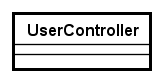
\includegraphics[scale=0.8]{UML/Classi/Back-End/QuizziPedia_Back-End_App_Controllers_UserController.png}
	\caption{QuizziPedia::Back-End::App::Controllers::UserController}
\end{figure}
\FloatBarrier
\begin{itemize}
	\item 
	\textbf{Descrizione}:
	classe che raggruppa attraverso require i vari \textit{controllers\ped{G}}  responsabili delle operazioni legate alla gestione degli utenti. Si è scelto di predisporre questo raggruppamento per facilitare l'introduzione di nuove funzionalità legate alla gestione degli utenti;
	\item \textbf{Utilizzo}:
	viene utilizzata per raggruppare i \textit{controllers\ped{G}}  responsabili della gestione dei dati degli utenti. In questo modo le classi che vogliono comunicare con i \textit{controllers\ped{G}}  legati agli utenti necessitano di includere solo questa classe e non ogni singolo controller;
	\item \textbf{Relazioni con altre classi}:
	\begin{itemize}
		\item 
			\textbf{IN	\texttt{UserRouter}}: 
			classe che gestisce le richieste relative alla registrazione e alla gestione della sessione di un utente. Componente ConcreteHandler del design pattern \textit{Chain of responsibility\ped{G}}. Utilizza il modulo \textit{Passport\ped{G}};		
		\item 
			\textbf{OUT \texttt{SessionController}}:
			classe \textit{middleware\ped{G}} che, utilizzando \textit{Passport\ped{G}}, si occupa di controllare la consistenza dell'oggetto session durante la sessione associata all'utente autenticato. È un componente ConcreteHandler del design pattern \textit{Chain of responsibility\ped{G}};
		\item 
			\textbf{OUT \texttt{AuthenticationController}}:
			classe che si occupa della registrazione e dell'autenticazione dell'utente nel sistema. È un componente ConcreteHandler del design pattern \textit{Chain of responsibility\ped{G}}. Risulta essere il componente che eventualmente esegue la richiesta del client attraverso \textit{Passport\ped{G}};	
		\item 
			\textbf{OUT \texttt{UserManagementController}}:
			classe che gestisce la logica applicativa riguardante la visualizzazione e la modifica dei dati dell'utente.
			Rappresenta il ConcreteHandler nel design pattern \textit{Chain of responsibility\ped{G}}. Utilizza \textit{Passport\ped{G}}.
	\end{itemize}
\end{itemize}
